\documentclass[10pt,a4paper]{amsart}
\usepackage[margin=19mm]{geometry}
\usepackage{amsmath,amssymb,mathtools}
\usepackage[scr=rsfs,cal=euler]{mathalfa}
\usepackage{xfrac}
\usepackage[unicode,hidelinks,bookmarks=false]{hyperref}
\newcommand{\ie}{i.e.\ }
\newcommand{\cf}{cf.\ }
\newcommand{\resp}{respectively\ }
\newcommand{\Subsection}{\subsection}
\providecommand{\nobreakdash}{\nobreak\hbox{-}}
\setlength{\emergencystretch}{2em}
\multlinegap0pt
\usepackage{tikz}
\usepackage{amssymb}
\usepackage[shortlabels]{enumitem}
\newtheorem{lemma}{Lemma}
\newtheorem{proposition}{Proposition}
\newtheorem{corollary}{Corollary}
\newtheorem{theorem}{Theorem}
\usepackage{cleveref}
\crefname{lemma}{Lemma}{Lemmas}
\crefname{proposition}{Proposition}{Propositions}
\crefname{corollary}{Corollary}{Corollarys}
\crefname{theorem}{Theorem}{Theorems}
\title{Periodic structure and Schr\"{o}dinger operators for codings of circle rotations}
\author{Luke Hetzel, Ronnie Pavlov}
\date{Source: arXiv:2609.00301v1 (CC BY 4.0)}
\begin{document}
\maketitle

\noindent\emph{Source and licence.} Periodic structure and Schr\"{o}dinger operators for codings of circle rotations. Version arXiv:2609.00301v1 (CC BY 4.0), distributed by arXiv under the Creative Commons Attribution 4.0 International licence, http://creativecommons.org/licenses/by/4.0/, as recorded in the arXiv licence metadata for this exact version and shown on the abstract page https://arxiv.org/abs/2609.00301v1. Full licence notice: \texttt{licenses/arxiv-2609.00301-CC-BY-4.0.txt}.\par\smallskip

\noindent\textit{Editorial scope.} Counted unit: the article's theorem onetwo (source0.tex lines 543--545). The article's complete original proof of it is delivered with it (source0.tex lines 547--871, one \texttt{proof} environment of 325 lines). No mathematics is written, repaired or re-derived: the statement and the proof are the article's own lines, in the article's own notation, and no retained line is substituted or re-flowed.  Retained uncounted as the source-local context the proof needs: lines 249--251; lines 262--264; lines 376--378; lines 472--474; lines 537--539.  Nothing was omitted from any retained span, so the package carries no omission record.  No retained line contains a citation, so the wrapper carries no bibliography and no bibliography entry.  The retained lines contain the article's own diagram code, which the wrapper typesets with the standard tikz packages; no image file is delivered and the package declares no asset dependency.  Editorial formatting only, in addition: an AMS \texttt{amsart} preamble that restates the article's own declarations and macros used by the retained lines, namely the environments \texttt{lemma}, \texttt{proposition}, \texttt{corollary}, \texttt{theorem} on separate counters, together with the standard packages those lines need.  The retained environments print in this document as Lemma 1, Proposition 1, Corollary 1, Theorem 1 in order of appearance, whereas the article prints the same items with the numbering of its own full document.  The complete native source of the article as distributed in the arXiv e-print for this exact version is bundled unchanged as \texttt{sources/209016/source0.tex}.
\begin{lemma}\label{qeps}
For any $\alpha$ and $k$, $q_k \epsilon_{k-1} < 1$ and $q_k \epsilon_k > (a_{k+1} + 2)^{-1}$. %$q_k (\epsilon_{k-1} + \epsilon_k) > (a_{k+1} + 2)^{-1}$.
\end{lemma}

\begin{lemma}\label{endpts}
If $q_k \alpha$ is positive, then $i\alpha$ is the left endpoint of a long gap in $Q_k$ iff $0 \leq i < q_{k-1}$. If $q_k \alpha$ is negative, then this characterizes right endpoints of long gaps. 
\end{lemma}

\begin{proposition}\label{longint}
For any $\alpha$ and $a$, if $\limsup \beta_k > 0$, then almost every $x \in X^{(I, \alpha)}$ has a shift with $3$-block Gordon structure.
\end{proposition}

\begin{equation}\label{uv}
U_k = \{j \alpha + \eta_k \ : \ i_k \leq j < q_k\} \textrm{ and } V_k = \{j \alpha + (q_k \alpha + \eta_k) \ : \ 0 \leq j < i_k\}.
\end{equation}

\begin{corollary}\label{bdaway}
If $\limsup a_k \leq 2$ and either $\liminf i_k/q_k < 0.0001$ or $\liminf d(a, Q_k)/\epsilon_k < 0.0001$, then almost all points of $X^{(I, \alpha)}$ have $3$-block Gordon structure.
\end{corollary}

\begin{theorem}\label{onetwo}
If $\limsup a_k = 2$ and $\liminf a_k = 1$, then almost every $x \in X^{(\alpha, I)}$ has a shift with $3$-block Gordon structure.
\end{theorem}

\begin{proof}
By the hypotheses of the theorem, there exists $K$ so that for $k > K$, $1 \leq a_k \leq 2$, and there are infinitely many values of $k$ for which $a_k = 1$ and for which $a_k = 2$. We can also assume (by increasing $K$ if necessary) that
$i_k/q_k, d(a, Q_k)/\epsilon_k \geq 0.0001$ for all $k > K$, since if this is not the case then the proof is complete by 
Proposition~\ref{longint} and Corollary~\ref{bdaway}. We assume for now that $q_k \alpha = \epsilon_k$ is positive without loss of generality.

Our proof relies on breaking into a variety of cases, and showing that each yields some $\beta_n$ bounded away from $0$, and then showing that this must happen infinitely many times. These cases will depend on whether $a$ is part of long or short intervals of length $S_k$ at various values of $k$. We remind the reader that by Lemma~\ref{endpts},
\begin{align*}
i \alpha \textrm{ is the left endpoint of a long interval in } Q_k & \Longleftrightarrow 0 \leq i < q_{k-1}\\
i \alpha \textrm{ is the right endpoint of a long interval in } Q_k & \Longleftrightarrow q_k - q_{k-1} \leq i < q_{k}.
\end{align*}
We refer to a value of $k$ when $a_{k+1} = 2$ as a $2$-split (since $\epsilon_{k-1} = 2\epsilon_{k} + \epsilon_{k+1}$, meaning that a short interval in $Q_k$ splits into two intervals, one long and one short, in $Q_{k-1}$) and a value of $k$ when $a_{k+1} = 1$ as a $1$-split for analogous reasons.\\
%(when $q_k \alpha$ is negative, this will characterize right endpoints, but we shouldn't need that fact.)\\

\noindent
\textbf{Case 1:} $a$ is part of a long interval for some $k > K$ with $a_{k+1} = 2$ (long gap before a $2$-split)\\

Suppose that this is the case. Then $i_k < q_{k-1}$, and based on the decomposition $Q_k + a = U_k \cup V_k$ from (\ref{uv}),
we see that all points of the form $j\alpha$ for $0 \leq j < i_k$ are shifted to the right by $\eta_k + \epsilon_k$, and all points of the form $j\alpha$ for $i_k \leq j < q_{k}$ are shifted to the right by $\eta_k$. %All of these points are left endpoints of long gaps by \Cref{endpts}).

Let us first suppose that $\eta_k \in (S_k, L_k) = (\epsilon_{k-1}, \epsilon_{k-1} + \epsilon_k)$. Then, consider all points $j\alpha$ for $q_{k-1} \leq j < (4/3)q_{k-1}$. These are all left endpoints of a short interval to the left of a long interval, meaning that $j\alpha + \eta_k$ will lie inside a long interval, at distance less than $\epsilon_k$ from the left endpoint. This implies that after its partition by points of $Q_k + a$, that long interval will still have a gap of length at least $S_k = \epsilon_{k-1} > 7/3 \epsilon_k$. Since there are $q_{k-1}/3$ such intervals, we see that by \Cref{qeps},
\[
\beta_k > (q_{k-1}/3)(\epsilon_k/3) > q_k \epsilon_k/27 > 1/108.
\]

We now assume that $\eta_k < S_k$. Then since $i_k/q_k > 0.0001$, we know that at least $0.0001q_k$ left endpoints of long gaps are shifted to the right by $\eta_k + \epsilon_k$. If $\eta_k > (7/6) \epsilon_k$, then this yields $0.0001q_k$ long gaps which retain an interval of length at least $(13/6) \epsilon_k$, which implies by \Cref{qeps} that
\[
\beta_k > (q_k/10000)(\epsilon_k/6) > q_k \epsilon_k/60000 > 1/240000.
\]
Before treating the final case $\eta_k \leq (7/6) \epsilon_k$, we note that $i_k$ cannot be too close to $q_{k-1}$: we can write
\[
-a = -i_k \alpha - \eta_k = (q_{k-1} - i_k) \alpha + (-q_{k-1} \alpha - \eta_k) = (q_{k-1} - i_k)\alpha + (\epsilon_{k-1} - \eta_k),
\]
corresponding to a decomposition of $-a$ as $i'_k \alpha + \eta'_k$ for $i'_k = q_{k-1} - i_k$ and 
$\eta'_k = \epsilon_{k-1} - \eta_k$. Since $Q_k \cup (Q_k - a) = T_k - a$ has exactly the same gaps as $T_k$, we may assume without loss of generality that $i'_k/q_k > 0.0001$ just as we did for $i_k$. In other words, we know that $i_k = q_{k-1} - i'_k < q_{k-1} - 0.0001q_k$. 

Now we treat the final case $\eta_k \leq (7/6) \epsilon_k$. By the bound just proved, there are at least $0.0001 q_k$ long intervals whose left endpoint is shifted to the right by $\eta_k$ in $Q_k + a$. Every such interval then retains a gap of length at least $L_k - (7/6)\epsilon_k > (13/6) \epsilon_k$ in $T_k$, which again implies by \Cref{qeps} that
\[
\beta_k > (q_k/10000)(\epsilon_k/6) > q_k \epsilon_k/60000 > 1/240000.
\]
We have then shown that in Case 1, $\beta_k > 1/240000$. 
\begin{flushright}
    $\square$\\
\end{flushright}

\noindent
\textbf{Case 2:} $a$ is part of a short interval for some $k > K$ with $a_{k+1} = 2$ and a long interval for $k+1$ 
(short gap before a $2$-split and long gap after)\\

\begin{figure}[h]
\centering
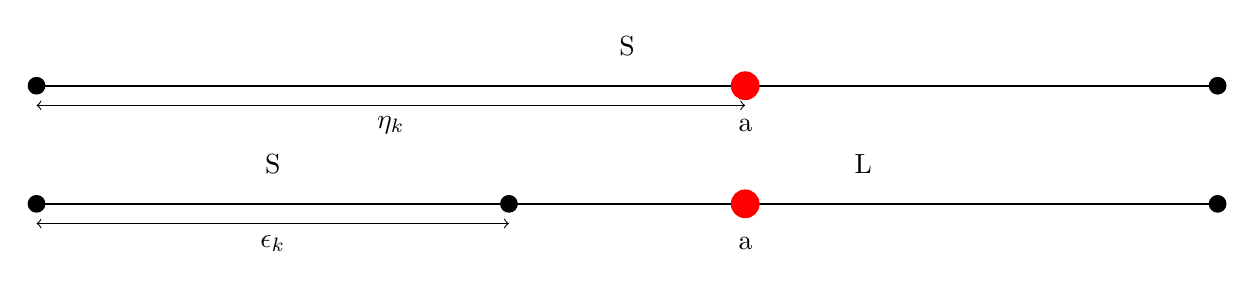
\begin{tikzpicture}
\draw[thick] (0,0) -- (15, 0);
\filldraw[black] (0,0) circle (3pt);
\filldraw[black] (15,0) circle (3pt);
\filldraw[red] (9,0) circle (5pt);
\draw[<->] (0, -.25) -- (9, -.25);
\node at (9,-0.5){a};
\node at (4.5,-0.5){$\eta_k$};
\node at (7.5,0.5){S};
\draw[thick] (0,-1.5) -- (15, -1.5);
\filldraw[black] (0,-1.5) circle (3pt);
\filldraw[black] (15,-1.5) circle (3pt);
\filldraw[black] (6,-1.5) circle (3pt);
\filldraw[red] (9,-1.5) circle (5pt);
\draw[<->] (0, -1.75) -- (6, -1.75);
\node at (3,-2){$\epsilon_k$};
\node at (9,-2){a};
\node at (3,-1){S};
\node at (10.5,-1){L};
\end{tikzpicture}
\caption{Case 2}\label{fig2}
\end{figure}

Suppose that this is the case. Since $a_{k+1} = 2$, the short interval $a$ lies in at step $k$ becomes a short interval to the left of a long interval in step $k+1$, and since $a$ is in the long interval there, $\eta_k$ must be greater than the length of a short interval at step $k+1$, which is $\epsilon_k$. In fact, then $\eta_k > \epsilon_k + 0.0001\epsilon_{k+1}$, by our assumption that $d(a, Q_{k+1})/\epsilon_{k+1} \geq 0.0001$. 

In addition, by Lemma~\ref{endpts}, $i_k \geq q_{k-1}$. This means that all points of the form $j\alpha + \eta_k + \epsilon_k$ for $0 \leq j < q_{k-1}$ are in $T_k$, meaning in turn that all long intervals in $Q_k$ are split by a point at least $\eta_k + \epsilon_k > 2\epsilon_k + 0.0001\epsilon_{k+1}$ from the left endpoint. Then by \Cref{qeps}, in Case 2,
\[
\beta_k > q_{k-1}(\epsilon_{k+1}/10000) > q_{k+1} \epsilon_{k+1}/90000 > 1/360000.
\]
\begin{flushright}
    $\square$\\
\end{flushright}

By Cases 1 and 2, we can assume WLOG that for $k > K$, $a$ is in a short gap before AND after every $2$-split.
(Otherwise the proof would be complete by \Cref{longint}.)
Consider any $k$ for which $a_{k+1} = 2$ and $a_{k+2} = 1$ (there are infinitely many of these). Then we know that $a$ was in a short interval at levels $k$ and $k+1$. The short interval from level $k+1$ becomes a single long interval at level $k+2$ since $k+1$ is a $1$-split. This means that $k+2$ cannot be a $2$-split, else we are in Case 1. Therefore, 
$a_{k+3} = 1$. \\

\noindent
\textbf{Case 3:} $a$ is part of a short interval at step $k+3$, $a_{k+1} = 2$, $a_{k+2} = a_{k+3} = 1$ 
(short, then short, then long, then short, for a $2$-split followed by two $1$-splits.)\\

\begin{figure}[h]
\centering
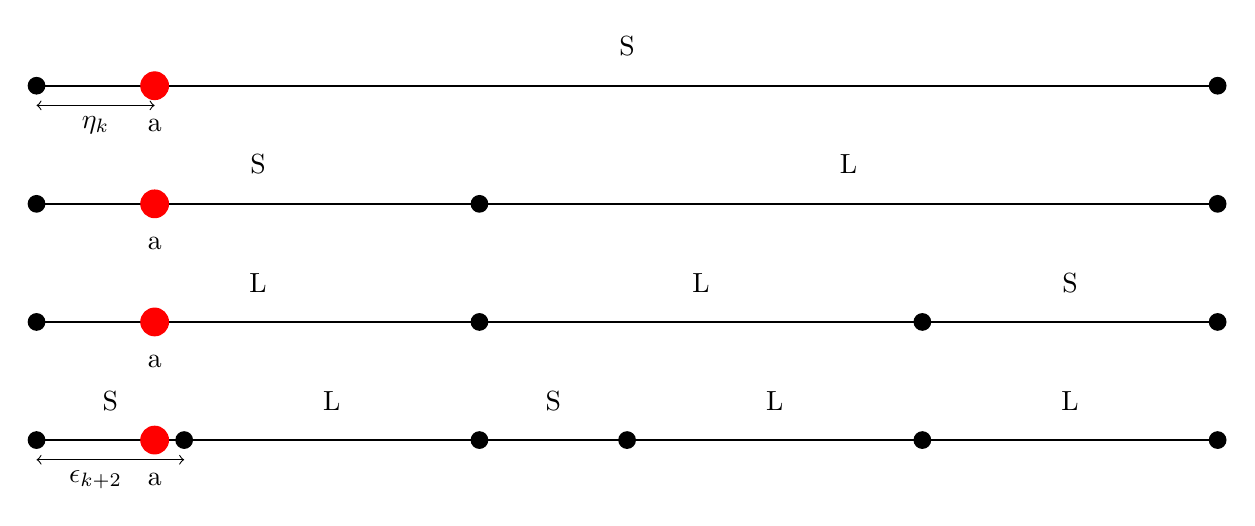
\begin{tikzpicture}
\draw[thick] (0,0) -- (15, 0);
\filldraw[black] (0,0) circle (3pt);
\filldraw[black] (15,0) circle (3pt);
\filldraw[red] (1.5,0) circle (5pt);
\draw[<->] (0, -.25) -- (1.5, -.25);
%\draw[<->] (0, -.25) -- (9, -.25);
\node at (1.5,-0.5){a};
\node at (0.75,-0.5){$\eta_k$};
\node at (7.5,0.5){S};
\draw[thick] (0,-1.5) -- (15, -1.5);
\filldraw[black] (0,-1.5) circle (3pt);
\filldraw[black] (15,-1.5) circle (3pt);
\filldraw[black] (45/8,-1.5) circle (3pt);
\filldraw[red] (1.5,-1.5) circle (5pt);
%\draw[<->] (0, -1.75) -- (6, -1.75);
%\node at (3,-2){$\epsilon_k$};
\node at (1.5,-2){a};
\node at (45/16,-1){S};
\node at (165/16,-1){L};
\draw[thick] (0,-3) -- (15, -3);
\filldraw[black] (0,-3) circle (3pt);
\filldraw[black] (15,-3) circle (3pt);
\filldraw[black] (45/8,-3) circle (3pt);
\filldraw[black] (45/4,-3) circle (3pt);
\filldraw[red] (1.5,-3) circle (5pt);
%\draw[<->] (0, -1.75) -- (6, -1.75);
%\node at (3,-2){$\epsilon_k$};
\node at (1.5,-3.5){a};
\node at (45/16,-2.5){L};
\node at (135/16,-2.5){L};
\node at (105/8,-2.5){S};
\draw[thick] (0,-4.5) -- (15, -4.5);
\filldraw[black] (0,-4.5) circle (3pt);
\filldraw[black] (15,-4.5) circle (3pt);
\filldraw[black] (7.5,-4.5) circle (3pt);
\filldraw[black] (15/8,-4.5) circle (3pt);
\filldraw[black] (45/8,-4.5) circle (3pt);
\filldraw[black] (45/4,-4.5) circle (3pt);
\filldraw[red] (1.5,-4.5) circle (5pt);
\draw[<->] (0, -4.75) -- (15/8, -4.75);
\node at (0.75,-5){$\epsilon_{k+2}$};
\node at (1.5,-5){a};
\node at (15/16,-4){S};
\node at (30/8,-4){L};
\node at (105/16,-4){S};
\node at (75/8,-4){L};
\node at (105/8,-4){L};
\end{tikzpicture}
\caption{Case 3}\label{fig3}
\end{figure}

The short interval $a$ lies in at step $k+3$ shares a left endpoint with the short interval from step $k$, and so $\eta_k$ is less than the length of a short interval at step $k+3$, which is $\epsilon_{k+2}$. Then as in Case 2, all left endpoints of long intervals at step $k$ get shifted to the right by $\eta_k + \epsilon_k$ in $Q_k + a$. This shift has length less than $\epsilon_k + \epsilon_{k+2}$. We note that by the standard recursions, the length of a long gap at level $k$ is
$\epsilon_{k-1} + \epsilon_k = 3\epsilon_k + \epsilon_{k+1} = 3\epsilon_k + \epsilon_{k+2} + \epsilon_{k+3}$. 

Therefore, all long gaps at level $k$ retain a gap of length $L_k - (\epsilon_k + \epsilon_{k+2}) = 2\epsilon_k + \epsilon_{k+3}$ in $T_k$. Therefore, by \Cref{qeps}, in Case 3 we have
\[
\beta_k > q_{k-1}\epsilon_{k+3} > q_k \epsilon_k/81 > 1/324.
\]
\begin{flushright}
    $\square$\\
\end{flushright}

The proof would be complete if Case 3 happened infinitely often, and so we can assume that for sufficiently large $k$, 
$a$ is part of a long interval at step $k+3$, implying that $a_{k+4} = 1$ (since we've assumed Case 1 does not occur for large $k$). We can then consider the position of $a$ starting from step $k+1$.\\

\noindent
\textbf{Case 4:} $a$ is part of a short interval at step $k+4$ and $a_{k+2} = a_{k+3} = a_{k+4} = 1$ 
(short, then long, then long, then short, for three $1$-splits)\\

\begin{figure}[h]
\centering
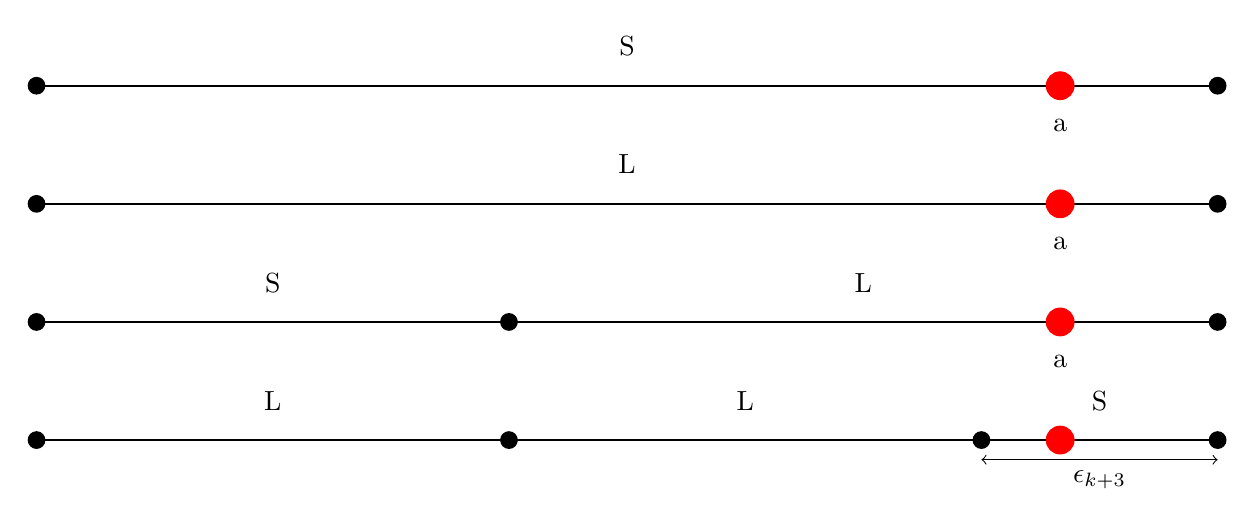
\begin{tikzpicture}
\draw[thick] (0,0) -- (15, 0);
\filldraw[black] (0,0) circle (3pt);
\filldraw[black] (15,0) circle (3pt);
\filldraw[red] (13,0) circle (5pt);
\node at (13,-0.5){a};
\node at (7.5,0.5){S};
%\draw[<->] (0, -.25) -- (1.5, -.25);
%\node at (0.75,-0.5){$\eta_k$};
\draw[thick] (0,-1.5) -- (15, -1.5);
\filldraw[black] (0,-1.5) circle (3pt);
\filldraw[black] (15,-1.5) circle (3pt);
\filldraw[red] (13,-1.5) circle (5pt);
%\draw[<->] (0, -1.75) -- (6, -1.75);
%\node at (3,-2){$\epsilon_k$};
\node at (13,-2){a};
\node at (7.5,-1){L};
\draw[thick] (0,-3) -- (15, -3);
\filldraw[black] (0,-3) circle (3pt);
\filldraw[black] (15,-3) circle (3pt);
\filldraw[black] (6,-3) circle (3pt);
\filldraw[red] (13,-3) circle (5pt);
%\draw[<->] (0, -1.75) -- (6, -1.75);
%\node at (3,-2){$\epsilon_k$};
\node at (13,-3.5){a};
\node at (3,-2.5){S};
\node at (10.5,-2.5){L};
\draw[thick] (0,-4.5) -- (15, -4.5);
\filldraw[black] (0,-4.5) circle (3pt);
\filldraw[black] (15,-4.5) circle (3pt);
\filldraw[black] (6,-4.5) circle (3pt);
\filldraw[black] (12,-4.5) circle (3pt);
\filldraw[red] (13,-4.5) circle (5pt);
\draw[<->] (12, -4.75) -- (15, -4.75);
\node at (13.5,-5){$\epsilon_{k+3}$};
%\node at (13,-5){a};
\node at (3,-4){L};
\node at (9,-4){L};
\node at (13.5,-4){S};
\end{tikzpicture}
\caption{Case 4}\label{fig4}
\end{figure}

We will end up showing that $\beta_{k+2}$ is bounded away from $0$ in this case, but first need to point out a new subtlety that arises since $a_{k+2} = 1$ (i.e. since we are making an argument at a value of $k$ corresponding to a $1$-split). Previously, as long as we could show that enough long gaps in $Q_k$ contained a point of $Q_k + a$ close to an endpoint, we were finished, because even though a second point of $Q_k + a$ could theoretically lie in that long interval, $S_k = \epsilon_{k-1} > (7/3) \epsilon_k$ was bounded away from $2\epsilon_k$, and so we were guaranteed a long enough interval in $T_k$. Now, $S_k < 2\epsilon_k$, so we need to take more care with this issue. 

In the situation of Case 4, $a$ is within distance $S_{k+4} = \epsilon_{k+3}$ of the right endpoint of the long interval $a$ lies in at level $k+2$. This means that we can, at level $k+2$, write $a = i\alpha + \eta$ for $-\epsilon_{k+3} < \eta < 0$. (This is not the standard representation of $a$ at level $k+2$, since $q_{k+2} \alpha$ is positive and $\eta$ is negative. But we will use it for this case only.) In fact we can say more; by assumption, $a$ is distance at least $0.0001\epsilon_{k+4}$ from all points in 
$Q_{k+4}$, and so $\eta > 0.0001\epsilon_{k+4} - \epsilon_{k+3}$. 

Since $a$ is near an endpoint of a long interval at level $k+2$ which was already in $Q_{k+1}$, we know that $i < q_{k+1}$. Using a similar argument with negating $a$ as in Case 1, we see that
\[
-a = -i\alpha - \eta = (q_{k+1} - i)\alpha + (-q_{k+1}\alpha - \eta) = (q_{k+1} - i)\alpha + (\epsilon_{k+1} - \eta).
\]
Since we assumed that $-a$ does not have a representation with infinitely many $i_k/q_k < 0.0001$, as before we know 
that $i < q_{k+1} - 0.0001 q_{k+2}$. 

Now, consider any point in $Q_k$ of the form $j \alpha$ with $q_{k+2} - q_{k+1} < j < 1.0001q_{k+2} - q_{k+1}$. This is the right endpoint of a long interval, and after adding $a$, it is $(j + i)\alpha + \eta$, which is a right endpoint of a long interval shifted to the left by $|\eta| < \epsilon_{k+3} - 0.0001\epsilon_{k+4}$. 

This means that it retains an interval of length at least 
\[
L_{k+2} - (\epsilon_{k+3} - 0.0001\epsilon_{k+4}) = \epsilon_{k+1} + \epsilon_{k+2} - \epsilon_{k+3} + 0.0001\epsilon_{k+4}
= 2\epsilon_{k+2} + 0.0001\epsilon_{k+4}.
\]

Since there were $0.0001q_{k+2}$ such intervals, by \Cref{qeps},
\[
\beta_{k+2} > (\epsilon_{k+4}/10000)(q_{k+2}/10000) > \epsilon_{k+2}q_{k+2}/400000000 > 1/1600000000
\]
in Case 4.
\begin{flushright}
    $\square$\\
\end{flushright}

The proof would again be complete if Case 4 occurred infinitely often, so for large $k$ we may assume that $a$ lies in a long interval at levels $k+2$, $k+3$, and $k+4$, and $a_{k+1}, a_{k+2}, a_{k+3} = 1$. Since $\limsup a_k = 2$, there must exist some $k' > k+2$ which is a $2$-split, implying that $a$ lies in a short interval at level $k'$ by Case 1. We may then take $k'$ to be the minimal value greater than $k+2$ where $a$ lies in a short interval, meaning that $a_{k'-2}, a_{k'-1}, a_{k'} = 1$ (and $a_{k'+1} = 2$).\\

\noindent
\textbf{Case 5:} $a$ is part of a long interval at levels $k' - 3$, $k' - 2$, $k' - 1$, and a short interval at level $k$
(long, then long, then long, then short, for three $1$-splits).\\

\begin{figure}[h]
\centering
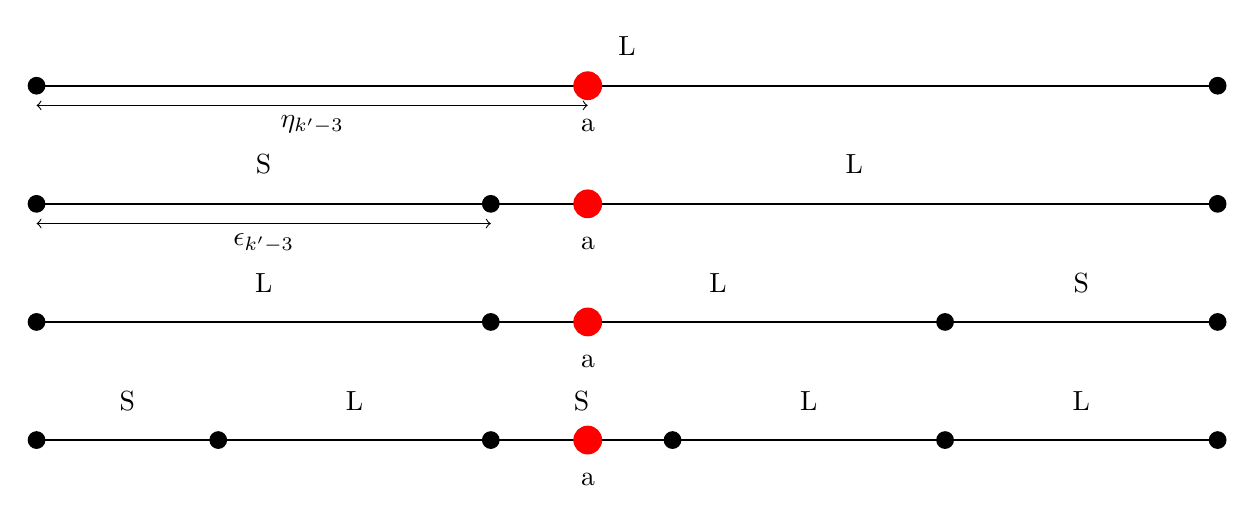
\begin{tikzpicture}
\draw[thick] (0,0) -- (15, 0);
\filldraw[black] (0,0) circle (3pt);
\filldraw[black] (15,0) circle (3pt);
\filldraw[red] (7,0) circle (5pt);
\node at (7,-0.5){a};
\node at (7.5,0.5){L};
\draw[<->] (0, -.25) -- (7, -.25);
\node at (3.5,-0.5){$\eta_{k'-3}$};
\draw[thick] (0,-1.5) -- (15, -1.5);
\filldraw[black] (0,-1.5) circle (3pt);
\filldraw[black] (15,-1.5) circle (3pt);
\filldraw[black] (75/13,-1.5) circle (3pt);
\filldraw[red] (7,-1.5) circle (5pt);
\draw[<->] (0, -1.75) -- (75/13, -1.75);
\node at (75/26,-2){$\epsilon_{k'-3}$};
\node at (7,-2){a};
\node at (75/26,-1){S};
\node at (135/13,-1){L};
\draw[thick] (0,-3) -- (15, -3);
\filldraw[black] (0,-3) circle (3pt);
\filldraw[black] (15,-3) circle (3pt);
\filldraw[black] (75/13,-3) circle (3pt);
\filldraw[black] (150/13,-3) circle (3pt);
\filldraw[red] (7,-3) circle (5pt);
%\draw[<->] (0, -1.75) -- (6, -1.75);
%\node at (3,-2){$\epsilon_k$};
\node at (7,-3.5){a};
\node at (75/26,-2.5){L};
\node at (225/26,-2.5){L};
\node at (172.5/13,-2.5){S};
\draw[thick] (0,-4.5) -- (15, -4.5);
\filldraw[black] (0,-4.5) circle (3pt);
\filldraw[black] (15,-4.5) circle (3pt);
\filldraw[black] (75/13,-4.5) circle (3pt);
\filldraw[black] (150/13,-4.5) circle (3pt);
\filldraw[black] (30/13,-4.5) circle (3pt);
\filldraw[black] (105/13,-4.5) circle (3pt);
\filldraw[red] (7,-4.5) circle (5pt);
%\draw[<->] (13, -4.75) -- (15, -4.75);
%\node at (14,-5){$\epsilon_{k+3}$};
\node at (7,-5){a};
\node at (15/13,-4){S};
\node at (105/26,-4){L};
\node at (90/13,-4){S};
\node at (255/26,-4){L};
\node at (172.5/13,-4){L};
\end{tikzpicture}
\caption{Case 5}\label{fig5}
\end{figure}

Since we know nothing about the parity of $k' - k$, here we cannot assume anything about the sign of $q_{k' - 3} \alpha$ without loss of generality. We still begin with the case where it is positive and then describe required changes in the opposite case.

Since $a$ lies in long intervals at levels $k'-3$, $k'-2$, $k'-1$, and short at $k'$, the short interval it lies in at level $k'$ shares left endpoint with the long interval from level $k'-2$. In addition, recall that $d(a, Q_{k'-2}) > 0.0001 \epsilon_{k'-2}$. Therefore, $\eta_{k'-3} \in (\epsilon_{k'-3} + 0.0001 \epsilon_{k'-2}, \epsilon_{k'-3} + \epsilon{k'-1})$. Since $a$ lies in a long gap at level $k'-3$, by Lemma~\ref{endpts} $i_{k'-3} < q_{k'-4}$. 

%Using a similar argument with negating $a$ as in Case 1, we see that
%\[
%-a = -i_{k'-3}\alpha - \eta_{k'-3} = (q_{k'-4} - i_{k'-3})\alpha + (-q_{k'-4}\alpha - \eta_{k'-3}) = 
%(q_{k'-4} - i_{k'-3})\alpha + (\epsilon_{k'-4} - \eta_{k'-3}).
%\]
%Since $\eta_{k'-3} < \epsilon_{k'-3} + \epsilon_{k'-1} < \epsilon_{k'-3} + \epsilon_{k'-2} = \epsilon_{k'-4}$, this is the correct representation for $-a$. Since we assumed that $-a$ does not have a representation with infinitely many $i_n/q_n < 0.0001$, as before we know that $i_{k'-3} < q_{k'-4} - 0.001 q_{k'-3}$. 

Now, consider any point in $Q_k$ of the form $j \alpha$ with $0.9999 q_{k'-3} < j < q_{k'-3}$. This is the right endpoint of a long interval, and after adding $a$, it is $(j + i_{k'-3} - q_{k'-3})\alpha + (\eta_{k'-3} + \epsilon_{k'-3})$, which is a left endpoint of a long interval shifted to the right by 
\[
\eta_{k'-3} + \epsilon_{k'-3} \in (2 \epsilon_{k'-3} + 0.0001\epsilon_{k'-2}, 2\epsilon_{k'-3} + \epsilon_{k'-1}).
\] 
This means that the corresponding long interval retains an interval of length at least $2\epsilon{k'-3} + 0.0001 \epsilon_{k'-2}$ in $T_k$. Since there are $0.0001 q_{k'-3}$ such intervals,
\[
\beta_{k'-3} > (\epsilon_{k'-2}/10000)(q_{k'-3}/10000) > \epsilon_{k'-3}q_{k'-3}/200000000 > 1/800000000.
\]

If instead $q_{k'-3} \alpha$ were negative, all left and right endpoints in the proof are swapped, and the sign of $\eta_{k'-3}$ will be negative, but nothing else needs to change. Therefore, in Case 5, $\beta_{k'-3} > 1/800000000$.
\begin{flushright}
    $\square$\\
\end{flushright}

Between any $k_1, k_2$ for which $a_{k_1} = a_{k_2} = 2$ and $a_{k_1 + 1} = a_{k_2 + 1} = 1$, one of Cases 1-5 must occur, and so there is a value of $k$ for which $\beta_k > 10^{-9}$. Since there are infinitely many such $k$, by Proposition~\ref{longint}, the proof is complete.

\end{proof}

\end{document}
